%iffalse
\let\negmedspace\undefined
\let\negthickspace\undefined
\documentclass[journal,12pt,twocolumn]{IEEEtran}
\usepackage{cite}
\usepackage{amsmath,amssymb,amsfonts}
\usepackage{graphicx}
\usepackage{textcomp}
\usepackage{xcolor}
\usepackage{txfonts}
\usepackage{listings}
\usepackage{enumitem}
\usepackage{mathtools}
\usepackage{gensymb}
\usepackage{comment}
\usepackage[breaklinks=true]{hyperref}
\usepackage{tkz-euclide} 
\usepackage{listings}
\usepackage{gvv}                                        
\def\inputGnumericTable{}                                 
\usepackage[latin1]{inputenc}                                
\usepackage{color}                                            
\usepackage{array}                                            
\usepackage{longtable}                                       
\usepackage{calc}                                             
\usepackage{multirow}                                         
\usepackage{hhline}                                           
\usepackage{ifthen}                                           
\usepackage{lscape}
\usepackage[export]{adjustbox}

\newtheorem{theorem}{Theorem}[section]
\newtheorem{problem}{Problem}
\newtheorem{proposition}{Proposition}[section]
\newtheorem{lemma}{Lemma}[section]
\newtheorem{corollary}[theorem]{Corollary}
\newtheorem{example}{Example}[section]
\newtheorem{definition}[problem]{Definition}
\newcommand{\BEQA}{\begin{eqnarray}}
\newcommand{\EEQA}{\end{eqnarray}}
\newcommand{\define}{\stackrel{\triangle}{=}}
\newtheorem{rem}{Remark}

\begin{document}
\parindent 0px
\bibliographystyle{IEEEtran}

\vspace{3cm}

\title{}
\author{EE23BTECH11042 -  Khusinadha Naik$^{*}$
}
\maketitle
\newpage
\bigskip

% \renewcommand{\thefigure}{\theenumi}
% \renewcommand{\thetable}{\theenumi}


\section*{Exercise 14}

\noindent \textbf{13.} \hspace{2pt}Figure 14.26 (a) shows a spring of force constant k clamped rigidly at one end and a mass m attached to its free end. A force F applied at the free end stretches the spring. Figure 14.26 (b) shows the same spring with both ends free and attached to a mass m at either end. Each end of the spring in Fig. 14.26(b) is stretched by the same force F


\begin{figure}[htbp]
    \centering
    \begin{subfigure}{\linewidth}
        \centering
        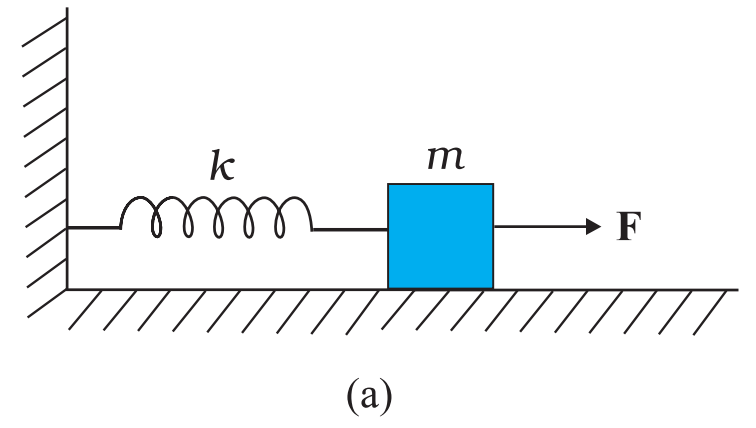
\includegraphics[width=0.3\textwidth]{./figs/fig1.png}

    \end{subfigure}
    \begin{subfigure}{\linewidth}
        \centering
        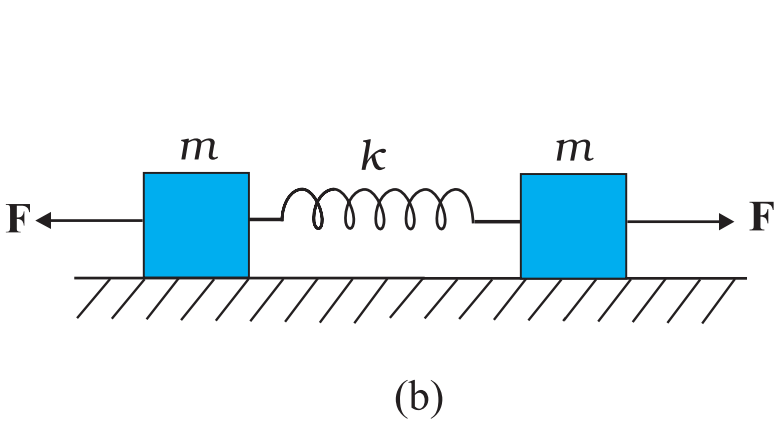
\includegraphics[width=0.3\textwidth]{./figs/fig2.png}

    \end{subfigure}
\end{figure}

\begin{enumerate}[label = (\alph*)]
	\item What is the maximum extension of the spring in the two cases ?		
	\item If the mass in Fig. (a) and the two masses in Fig. (b) are released, what is the
period of oscillation in each case ?
\end{enumerate}


\end{document}


\end{document}
